\section{Geoscape}

\subsection{Worldmap - an overview}
Welcome to Geoscape! As noted previously, UFO:AI distinguishes between two major aspects of the game -- macromanagement and tactical combat. While combat is where you earn the bucks, this is where you spend them.

\emph{Geoscape} is itself made up of two screens. The first is the world map, which is the first screen you will see right after starting a new campaign. It is used to get the big picture of world events, as well as coordinating combat missions and intercepting enemy UFOs. The other screen is the base overview, where you improve base infrastructure and implement decisions about equipment, research, and production. In the following sections we will take a closer look at both of these screens.

The following screenshot shows the uses to which we can put the world map. You can see that it is divided into day and night zones, which influences any combat missions you get into.  The day/night borderline also changes shape according to the seasons as the relation of the Earth to the Sun changes.\\

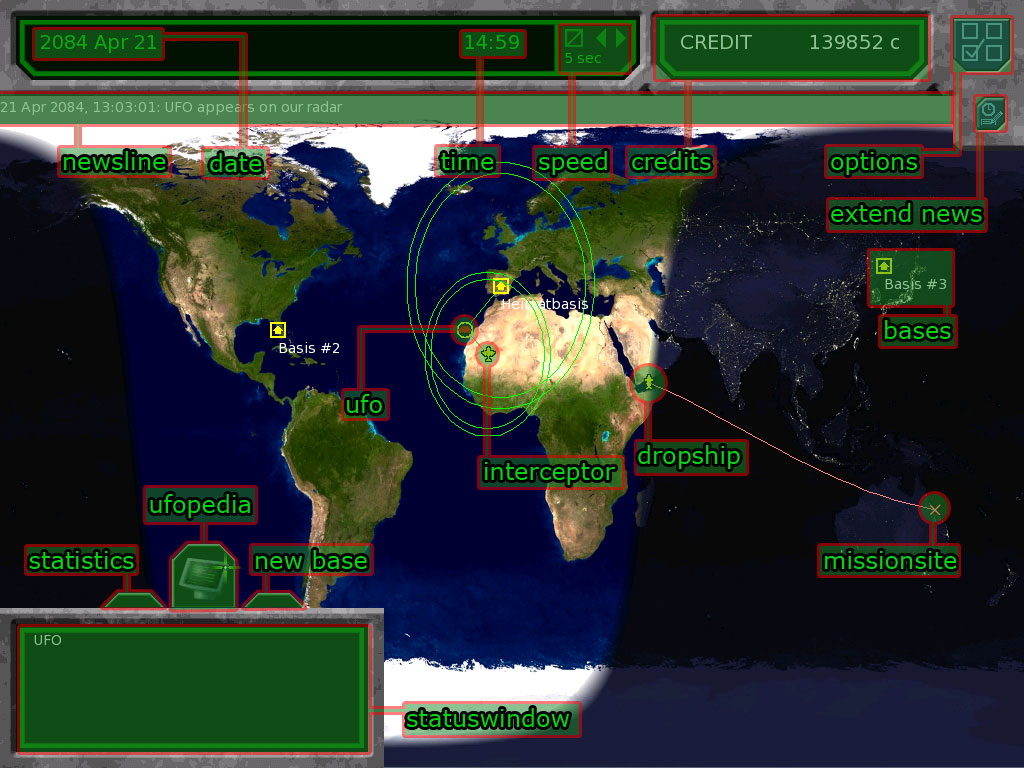
\includegraphics[width=\textwidth]{images/geoscape_final.jpg}

\newpage

\subsubsection{Status Window}
Here some general information like stats and descriptions will show up, depending on context.

\subsubsection{Statistics}
If you hover over the registers in the bottom left, three different buttons will show up. The leftmost leads to some more detailed statistics about your attempt to save the world. In addition to more general information (like missions won/lost etc.) you can also find out about the attitude of all the UN countries paying you. You should be aware that if you fail to protect particular countries from alien invasions (maybe because your infrastructure is not well established in that region) they will cut the resources they provide -- both financial and potential employees.

\subsubsection{Ufopedia}
The middle button is the Ufopedia, a comprehensive collection of useful information about items, technologies, damage types and so on. As your research proceeds, the Ufopedia grows as well, so make sure you check out the latest information  every now and then.

\subsubsection{New base}
The rightmost button allows you to establish a new base anywhere on the planet's landmass. A new base, once you have built it up, can give additional radar range, research and production capacities, as well as new hangars for your aircraft.  There is no practical difference between your first base and ones you build subsequently.

\subsubsection{Date}
This gives you the current date, so you know when it's close to pay day. You should also keep an eye on the date because while you -- in principle -- have unlimited time to play the game, the aliens get stronger and better equipped as the game proceeds. It is in humanity's best interest if you can catch up with them sooner than later in order to save your beloved homeworld.

\subsubsection{Time and Game Speed}
This is where you can adjust the gamespeed from 5secs all the way through to steps of one day. Whatever this is set to, while you are in combat time is stopped and it will be all the same when you return from battle.  The game will also automatically pause for certain events like UFO spottings and landings.

\subsubsection{Credits}
Never forget that you can't spend what you don't have.  This shows your available cash.

\subsubsection{Options}
Gets you to the \emph{Options} menu where you can load and save your game as well as start a new one.
Through \textbf{exit} you reach the main menu where you can change game settings and continue your current game (via Single Player $\rightarrow$ Continue)

\subsubsection{News and extended news}
The permanent news line in the upper left always represents the latest news (such as promotions, cashflow, UFO sightings and attacks) while the \emph{extended news} button pops up a list of the last 20 new lines.  Whenever you notice news, you should check the button as well so as not to miss anything.

\subsubsection{Bases}
The yellow houses represent your bases. Circles around them represent the range of their radars. To bring up the base view, just click on its symbol.

\subsubsection{Your ships}
You have two general classes of ships, interceptors and dropships.  Both work the same.  While they're out on mission, a single click will select them, and clicking somewhere on the map orders them to move there.  A doubleclick brings up a window for more advanced orders.  Interceptors are used for intercepting and shooting down UFOs, while dropships are used to get your soldiers out on a mission.  Your ships have limited ranges, which you may extend by supplying them with extra fuel tanks.  However, the tanks will slow down the ships.

% Is this the right section name?  Talk about how these are displayed, maybe with a screenshot.
\subsubsection{Upcoming missions}
This is where the action waits. Selecting a mission will give you a short description on the status screen while a second one allows you to select a ship to bring in the troops you want.
